\documentclass[12pt,a4paper, french]{article}
\usepackage{natbib}         % Pour la bibliographie
\usepackage{url}            % Pour citer les adresses web
\usepackage[T1]{fontenc}    % Encodage des accents
\usepackage[utf8]{inputenc} % Lui aussi
\usepackage{babel} % Pour la traduction française

\usepackage{graphicx}
\graphicspath{ {./src/} }

% Mettez votre titre et votre nom ci-après
\title{Rapport de TIPE Sup \\
Reconnaissance vocale lors d'appel d'urgence grâce à un réseau de neurones}
\author{Tran-Thuong Tien-Thinh, MPSIA, 2020-2021}
\date{}

\begin{document}

\maketitle

\begin{abstract}
D'après les chiffres du ministère, il y a eu plus de 31 millions d'appels d'urgence en 2019. Ces appels sont réparties sur 103 centres de plus en plus sollicités. Alors que les recommandations fixe un taux de 90\% de réponses en moins de 60 secondes, seul 69\% des appels étaient décrochés dans la minute.  

Afin de répondre à ce problème, nous nous proposons d'étudier une intelligence artificielle capable de faire de la reconnaissance vocale, pour alléger le travail des opérateurs d'appel d'urgence.
\end{abstract}

\section*{Problématique retenue}
\noindent\textit{INFORMATIQUE (Informatique Pratique)}

Il s’agit de concevoir un réseau de neurones capable de reconnaitre la voix pour retranscrire ce qui est prononcé et de classer le niveau d'urgence d'un appel.

\section*{Objectif TIPE du candidat}
\begin{enumerate}
    \item Faire un réseau de neurones qui converge grâce à l’algorithme du gradient
    \item Améliorer la vitesse d'entrainement grâce à des optimizers basés sur la descente de gradient
    \item Essayer ce réseau sur la base de données du MNIST pour reconnaitre des chiffres
    \item Utilisation du transfert d'apprentissage pour reconnaître le nom de la personne qui a été prononcé dans un audio
\end{enumerate}

\section{Un réseau de neuronne simple imitant l'opérateur XOR}
La difficulté de l'opérateur XOR est qu'il n'effectue pas une classification linéaire entre les deux entrées :
\begin{center}
\begin{tabular}{ |c|c||c|   }
 \hline
 \multicolumn{3}{|c|}{Tableau de l'opérateur XOR} \\
 \hline
 Entrée 1 & Entrée 2 & Sortie\\
 \hline
 0 & 0 & 0\\
 1 & 0 & 1\\
 0 & 1 & 1\\
 1 & 1 & 0\\
 \hline
\end{tabular}
\end{center}

\subsection{Réseaux de neurones}
Il est possible de démontrer que la taille minimum du réseau de neuronne est 2 entrées, 2 neuronnes cachées et 1 neuronne en sortie.  

Pour améliorer la vitesse d'apprentissage il est possible d'utiliser des fonctions d'activation permettant de normaliser les sorties de chaque neuronne entre $[0, 1]$, comme la fonction \textit{sigmoïde}.
\begin{equation}
	\sigma(x) = \frac{1}{1+e^{-x}}
\end{equation}

\begin{center}
    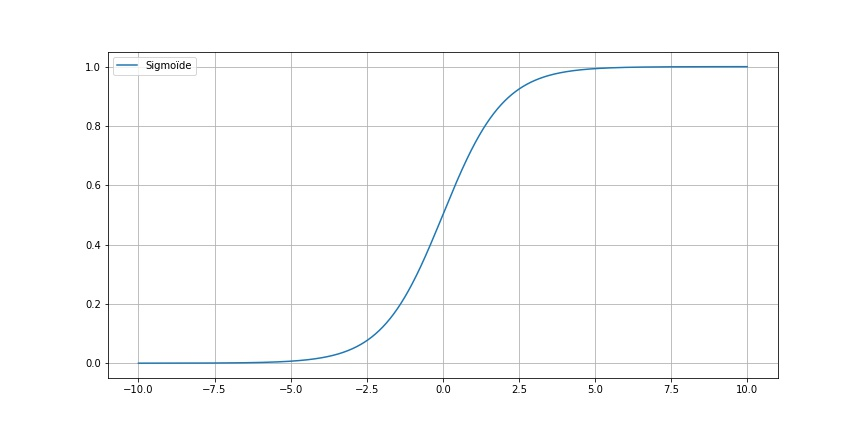
\includegraphics[height=4cm]{1-trace sigmoid.jpg} \\
    Courbe de la fonction d'activation sigmoïde
\end{center}


\subsection{Apprentissage}
Pour l'apprentissage des poids sur chaque neurone, il calculer l'erreur, et utiliser l'algorithme de rétropropagation. Un des moyen pour calculer la différence à appliquer au poids par rapport à l'erreur $\frac{d_{erreur}}{d_w}$ est la descente de gradient.

\begin{equation}
	\frac{d_{erreur}}{d_{poids}} = 
		\frac{d_{erreur}}{d_{\sigma(sortie)}} 
		\times 
		\frac{d_{\sigma(sortie)}}{d_{sortie}} 
		\times 
		\frac{d_{sortie1}}{d_{poids}}   
\end{equation}
\begin{equation}
	\frac{d_{erreur}}{d_{poids}} = 
		2(\sigma(sortie) - sortie_{cible})
		\times 
		\sigma'(sortie)
		\times 
		entree  
\end{equation}

\subsection{Resultats}
Le réseau de neurones indique bien les résultats associés au XOR :
\\
\noindent 
\textsf{
Les entrées [0, 0] donnent en sortie 0.03356776609399469 \\ 
Les entrées [1, 0] donnent en sortie 0.9295281916216991  \\
Les entrées [0, 1] donnent en sortie 0.9295281849281336  \\
Les entrées [1, 1] donnent en sortie 0.09395448088880454  \\
}

Le temps d'apprentrissage semble cependant avoir été très long, l'apprentissage a pris près de 10 000 époques d'apprentissage avant de converger vers un résultat d'erreur inférieur à 10\%.

\section{Optimizers}
Une des principale façon d'accélérer la vitesse d'apprentissage des neuronnes est l'utilisation des optimizers améliorant la descente de gradient simple.

\subsection{Regroupement des données par paquet (batch)}
Pour améliorer la vitesse d'apprentissage il est intéressant de grouper les données d'apprentissage par paquet (batch) et de mettre à jour le poid des neurones seulement après avoir évaluer la sortie pour chaque paquet de données. On réduit ainsi d'une part le nombre de mise à jour des poids, et on évite également l'influence de données abherrantes.  

Afin de choisir rapidement par combien nous regroupons les données il est fortement conseiller de procéder par dichotomie en fonction du nombre de données que l'on possède avec des paquets de $\{64; 128; 256; 512\}$ choisi à chaque fois aléatoirement.

\subsection{Moment}
Le moment permet d'accentuer la modification des poids lorsque plusieurs données d'affilées génèrent les mêmes modification de poids. Cela permet de de faire varier le taux d'apprentissage (learning rate) en fonction des modifications passées.

Au lieu de modifier directement le poids des neurones avec la formule :
\begin{equation}
	poids \leftarrow
	poids - taux_{apprentissage} \times d_{poids}
\end{equation}

On prend en compte les poids passées avec la formule avec $\gamma = 0.5$ le taux de prise en compte du moment précédent :
\begin{equation}
	d_{moment} \leftarrow 
	\gamma * d_{moment} + taux_{apprentissage} * d_{poids}
\end{equation}
\begin{equation}
	poids \leftarrow
	poids - d_{moment}
\end{equation}


Le moment permet également de sortir des problèmes possédant des solutions locales non optimales.


\section{MNIST reconnaissance de chiffre écrit à la main}
En utilisant tout ce que j'ai fait ci-dessus, j'ai créer un réseau de neuronne capable de reconnaitre des chiffres écrit à la main. Comme c'est un problème de classification avec $10$ classes différentes $[|0; 9|]$, il est plus intéressant d'utiliser une fonction d'activation \textit{softmax} plutôt que sigmoïde :  
\begin{equation}
	\sigma(X)_i = \frac{e^{X_i}}{\sum_{j=0}^{9}{e^{X_j}}} 
	\quad \textrm{avec} \quad
	\textrm{X la matrice colonne des 10 sorties}
\end{equation}

\subsection{Résultat}
Les résultats sont intérressant, plus de 95\% de bonne réponses sur les données de test, mais il a fallu l'entrainer pendant près de 500 époques (50 minutes environ) d'apprentissage.

J'ai donc appliqué l'optimizer avec le moment décrit plus tôt sur les 50 premières époques et on remarque bien un apprentissage plus rapide lors des 10 premières époques.


\section{Classification d'audio }
Mon projet final est de classifier des séquende d'audio. J'ai donc essayé de faire un réseau de neurones capable de reconnaître le nom de mes professeurs \{"Bensal", "Châteaux", "Gayout", "Le Grandic", "Mistler", "Schuschu"\}. Pour cela j'ai décomposé l'audio avec la transformée de Fourier pour avoir un spectrogramme de celui-ci.

\begin{center}
    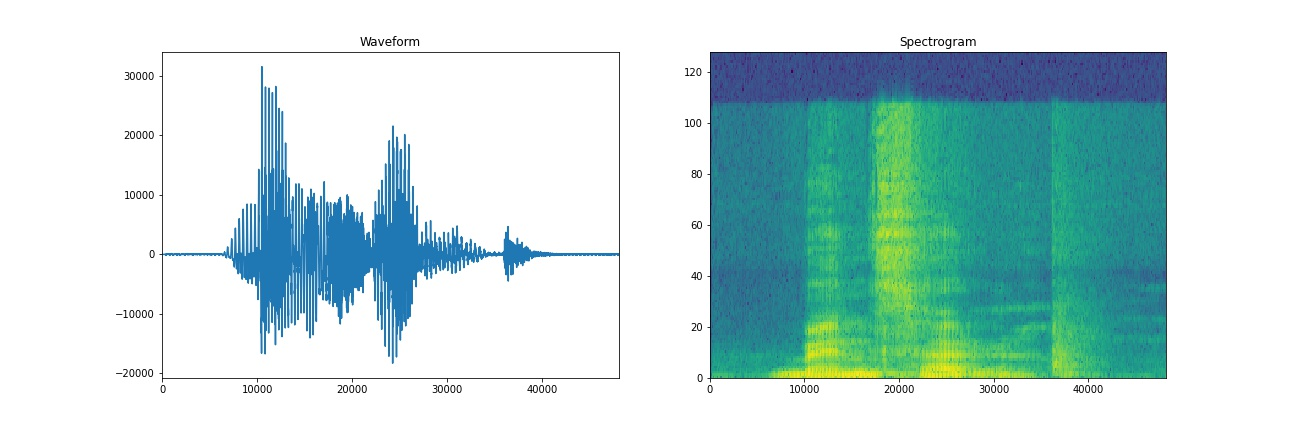
\includegraphics[width=13cm]{4-Audio Bensaal.jpg} \\
    Un audio "Bensal" et sa décomposition \textit{Short-time Fourier transform}
\end{center}

\subsection{Transfert d'apprentissage}
\textit{Cette section utilise la librairie Tensorflow pour la création et l'entrainement des réseaux de neurones.}  
  
J'ai entrainé un model sur une base de données de Google avec les mots \{"down", "go", "left", "no", "right", "stop", "up", "yes"\} afin de lui permettre de reconnaître des sons caractéristiques avec le plus données possible. Le model était ensuite entrainé, j'ai extrait de ce model les premières couches de neurones et j'ai fixé leurs poids. J'ai ensuite rajouté des neurones permettant à partir des sons caractéristiques reconnus de reconnaitre les noms qui sont prononcés.
\begin{center}
    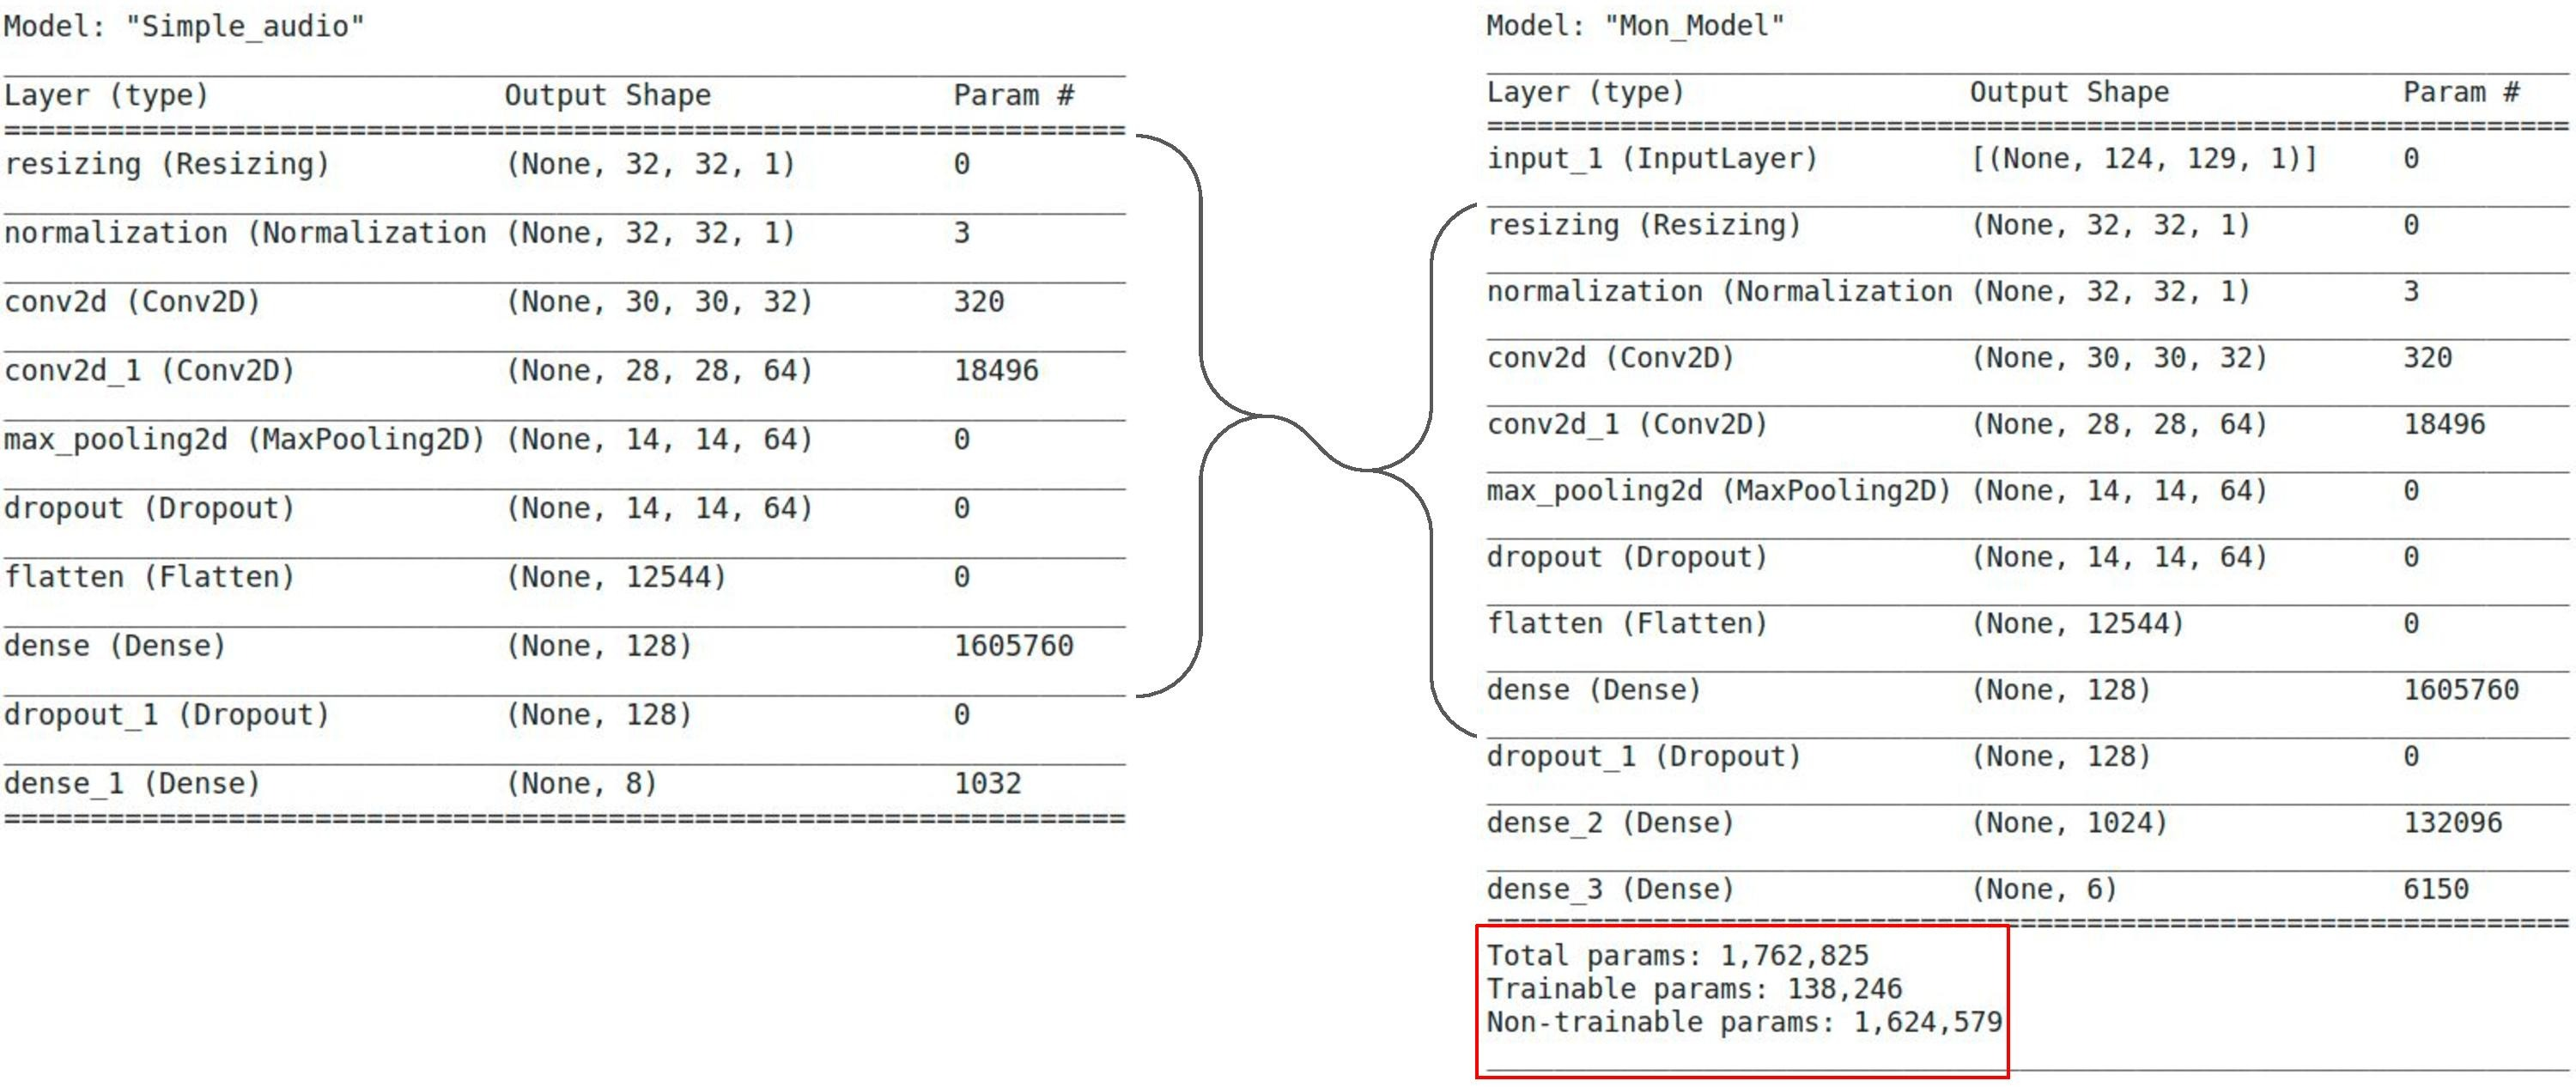
\includegraphics[width=12cm]{4-Transfert Learning.jpg} \\
    Transfert des couches de \textit{Simple audio} vers \textit{Mon model}
\end{center}

\subsection{Augmentation de données}
Je me suis enregistré Agathe et moi en train de dire le nom de nos 6 professeurs 8 fois chacun. Etant donné qu'il fallait beaucoup plus de données, j'ai fait de l'augmentation de données (petites modifications des données permettant d'avoir plus de données différentes) :  
\begin{enumerate}
	\item Ajout de bruit $\times 4$
	\item Modulation de la voix (grave, aigu) $\times 4$
	\item Modulation de la vitesse du son $\times 4$
	\item Découpage du son $\times 4$
\end{enumerate}
Ce qui me permet de me retrouver avec $4^4 = 256$ fois plus de données différentes. Ainsi je me retrouve avec $256 \times 8 \times 2 = 4096$ audios.

\subsection{Résultat}
Les résultat sont concluant, il y a plus de 80\% de bonnes réponses lorsque c'est Agathe ou moi qui utilisons testons le réseau de neurones. Ce taux de exactitude est réduit en fonction de la voix et l'intonation de la personne qui teste le model. 

\begin{center}
    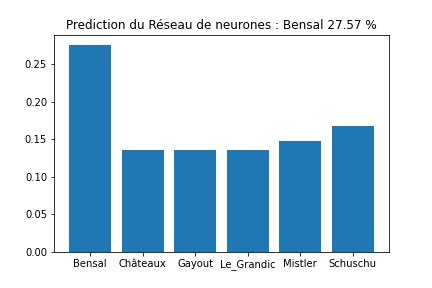
\includegraphics[width=12cm]{4-Resultat Bensal.jpg} \\
    Prediction pour un audio où "Bensal" a été prononcé
\end{center}

\section*{Annexes}
Tous mes codes : github.com/tttienthinh/4Tipe


\end{document}